%% Right Answer, Wrong Analysis?
%% WSDM 2027 submission. Every number in this file is emitted by
%%     python scripts/paper_numbers.py
%% and every figure by scripts/figure1.py and scripts/figure2.py, both of which read the run
%% data directly. If a number appears here and not in that output, it is unverified.
\documentclass[sigconf,anonymous,review]{acmart}

\AtBeginDocument{%
  \providecommand\BibTeX{{Bib\TeX}}}
\setcopyright{none}
\acmConference[WSDM '27]{Proceedings of the 20th ACM International Conference on Web Search and
  Data Mining}{March 2027}{}
\settopmatter{printacmref=false}
\renewcommand\footnotetextcopyrightpermission[1]{}
\pagestyle{plain}

\usepackage{booktabs}
\usepackage{amsmath}
% amssymb is NOT loaded: acmart's newtxmath already provides \mathbb,
% and loading it clashes on \Bbbk.
\usepackage{graphicx}
\usepackage{xcolor}

\newcommand{\pairacc}{\textsc{PairAcc}}
\newcommand{\evpair}{\textsc{EVPairAcc}}
\newcommand{\Gp}{\mathcal{G}^{+}}
\newcommand{\Gm}{\mathcal{G}^{-}}

\begin{document}

\title{Capability Is Not Validity:\\
       Evaluating Agentic Temporal Graph Analysis}

\author{Anonymous Author(s)}

\begin{abstract}
Large language model agents increasingly analyze structured data through adaptive sequences of tool
calls, yet final-answer accuracy cannot reveal whether the interface exposed the needed
information, whether the model reconstructed it, or whether the computation the agent cites answers
the question that was asked. We introduce a controlled framework separating the effective
\emph{capability} of a model--interface pair from the \emph{evidence validity} of its successful
analyses, using a deterministic checker and no LLM judge. Temporal graphs make both measurable:
matched counterfactual worlds hold the node set, static edge multiset, event count and timestamp
multiset fixed while reversing temporal truth.

Across four mechanisms, four interface levels and five models ($1{,}402$ scored runs) the two
dimensions come apart. On a compound workload whose matched worlds each satisfy \emph{both}
component predicates and differ only in their temporal composition, \texttt{gpt-5-mini} answers
every pair correctly through semantic temporal operators (pair accuracy $1.00$) while no pair
is supported by cited computations that could distinguish the two worlds: evidence-valid pair
accuracy $0.00$. Capability varies independently: a primitive aggregate interface yields model- and
resource-dependent frontiers that a sandboxed interpreter removes, and that nuisance activity or a
four-fold larger graph reinstates. Agentic analytical systems must therefore be evaluated on two
axes: what they can do, and whether their successful analyses are valid.
\end{abstract}

\keywords{agentic data analysis, temporal graphs, LLM agents, tool interfaces, evaluation}

\maketitle

%% ===================================================================================
\section{Introduction}

Large language models are increasingly deployed as analytical agents rather than one-shot query
generators. Instead of translating a request into a single SQL or graph query, an agent inspects
intermediate results, chooses the next tool, refines a time window, executes code over raw events,
invokes a semantic operator, and combines several observations before concluding. The resulting
system is not just a language model: its behavior emerges from the interaction of the model, the
data interface, the execution environment, and the interaction budget. Temporal interaction graphs
underlie many workloads of interest to this community, including information diffusion, coordinated
behavior, evolving communities and social-network dynamics, which makes them a natural setting for
studying analytical agents over structured Web data.

Most evaluations collapse that process into one question: \emph{did the agent return the correct
answer?} For analytical systems this is necessary but not sufficient, because two agents that
answer identically may have done entirely different things. One may have recovered event times
through dozens of aggregate queries, another written a program over raw events, a third called a
semantic operator. More sharply, a semantic operator can execute perfectly and return the correct
result \emph{for the operation it was asked to perform}, yet still fail to establish the claim the
user intended. The agent may have omitted a waiting bound, widened an admissible interval, or
otherwise changed the proposition under test. We therefore treat two questions as independent
evaluation axes:

\begin{quote}
\textbf{Capability.} What can the model--interface system actually do?\\
\textbf{Validity.} When it succeeds, does the supporting computation establish the intended claim?
\end{quote}

\paragraph{A controlled microscope.}
Temporal graphs make both measurable. Consider two worlds with identical nodes, identical static
edges, identical event counts and identical timestamp multisets. In one, the timestamps along a
path satisfy an ordering and a waiting bound; in the other the same events and the same timestamps
are re-assigned so the static path survives but the bounded temporal path does not. An
order-oblivious interface cannot separate them. An interactive aggregate interface may expose the
distinction only indirectly. A programmable interface hands over raw events. A semantic interface
computes the target relation directly. Matched counterfactuals therefore isolate \emph{where the
analytical information enters the system, and what the agent must do with it}, and because any
strategy keyed on activity volume, node popularity or static connectivity returns the same value on
both worlds, such shortcuts score zero by construction rather than by instruction.

\paragraph{The result that motivates the paper.}
Our compound workload asks whether a closure wave completes at $t_c$ and a bounded cascade then
begins within $[t_c, t_c+\Delta_{\text{adm}}]$. Both matched worlds contain \emph{both} component
predicates, individually satisfied; they differ only in whether the cascade falls inside the
admissible interval. Given semantic temporal operators, \texttt{gpt-5-mini} answers every pair
correctly: pair accuracy $1.00$, in $2.4$ tool calls. Yet \emph{not one} of those answers is
supported by a cited computation capable of telling the two worlds apart. Its evidence-valid pair
accuracy is $0.00$. It queries an interval wider than the admissible lag, which returns
\emph{reachable} in both worlds by construction, and then reaches the right conclusion by reasoning
over the returned arrival times in prose (Figure~\ref{fig:one}). The composition is real, but it
lives in natural language and never in the computation the answer cites, and final-answer accuracy
cannot see the difference:
\begin{equation}
\text{correct answer} \;\not\Rightarrow\; \text{valid analysis.}
\end{equation}

\paragraph{Capability varies too, and not where one expects.}
The capability axis is equally uneven. We began with an interface exposing only filtered event
counts over chosen windows, with no timestamps, no ordering primitive and no path operator, and
expected it to be insufficient for temporal-order reasoning. A frontier model defeated that
expectation, repeatedly narrowing node-filtered windows to localize events and comparing the
recovered order: the interface has no ordering operation, yet ordering became effectively available
through adaptive composition. That capability then has a frontier. Holding the budget fixed and
growing the temporal search range, accuracy falls from $1.00$ to $0.00$ while the model keeps
attempting the same strategy in $80$--$100\%$ of runs, so what degrades is completion rather than
discovery. Exposing raw events with a sandboxed interpreter removes the frontier entirely, which
localizes it to information acquisition rather than to temporal reasoning; a nuisance-activity
overlay or a four-fold larger graph brings it back. Across three open-weight checkpoints the
frontier does not move with model size at all, which is why we describe strategy regimes rather
than a capability ordering.

\paragraph{Contributions.}
\begin{enumerate}
\item \textbf{Evidence-valid analytical correctness.} We define and operationalize \evpair{}, which
requires paired answers to be correct \emph{and} supported by a decisive cited computation that
preserves the task's semantic constraints. It is deterministic; no LLM judge is used anywhere.
\item \textbf{A staged model--interface capability profile} separating information availability,
strategy formation, execution, \emph{evidence interpretation}, semantic validity, and cost. The
interpretation stage is forced by our data rather than postulated.
\item \textbf{Capability-frontier evidence} across four mechanisms, four interfaces, budgets,
resolutions and five models, including a programmable baseline that localizes the frontier as
acquisition-induced and robustness cells that move it.
\item \textbf{A matched temporal counterfactual methodology} that controls declared nuisance
statistics exactly, enabling process-level diagnosis of \emph{why} an agent succeeded or failed.
\end{enumerate}


\begin{figure*}[t]
  \centering
  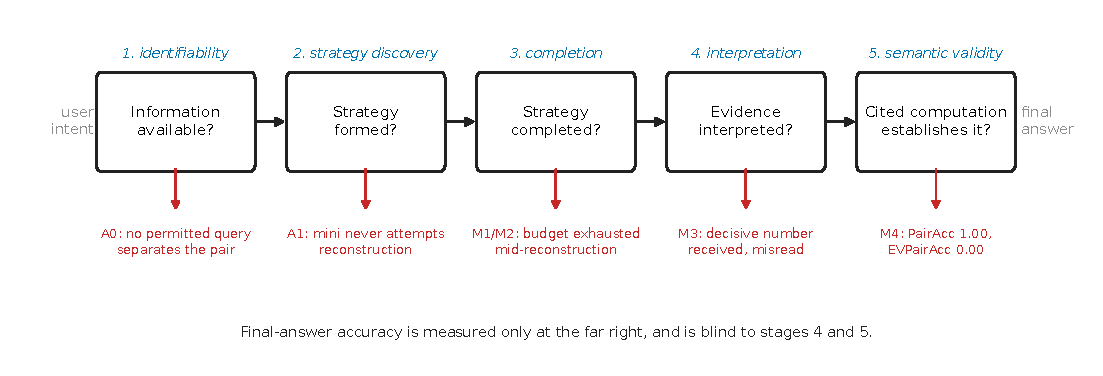
\includegraphics[width=\textwidth]{figures/figure_framework.pdf}
  \caption{\textbf{Capability and validity fail at different stages of agentic analysis.} Each
  stage can fail on its own, and each is exposed by a different part of our design. Final-answer
  accuracy observes only the right-hand end of the chain, which is why a system can be perfect
  there while failing at stage 4 or 5.}
  \label{fig:framework}
\end{figure*}

%% ===================================================================================
\section{Related Work}

\paragraph{Agent interfaces and abstraction.}
The interface through which an agent acts is increasingly treated as part of the agent system
rather than an implementation detail. SpatialClaw argues that action-interface design materially
alters spatial-reasoning capability and favors flexible, persistent composition over rigid
one-shot interfaces~\cite{spatialclaw2026}. The Declarative Model Interface similarly moves
low-level computer interaction out of the LLM and reports substantial gains from an interface
designed around model rather than human interaction~\cite{dmi2026}. Conversely, \emph{Terminal
Agents Suffice} shows that sufficiently capable coding agents can perform complex enterprise
workflows through low-level terminal and programmatic APIs, sometimes matching or outperforming
more elaborate abstractions~\cite{terminalagents2026}; tool-program interfaces explore the space
between fixed endpoints and unrestricted code by letting agents compose service operations
procedurally~\cite{toolprograms2026}. Together these establish that abstraction and programmability
strongly affect agent performance. \textbf{We do not claim that observation as new.} Our focus is
how to \emph{measure} what an interface makes effectively available to a particular model: whether
a task distinction is observable at all, whether the model discovers a strategy to recover it,
whether that strategy completes under a resource budget, and whether a successful computation
preserves the semantics of the intended claim.

\paragraph{Agentic graph and temporal-graph analysis.}
LLM4DyG evaluates spatial-temporal reasoning on dynamic graphs including chronological and
evolving-structure tasks~\cite{llm4dyg2024}; LLMTM evaluates temporal-motif analysis and develops a
tool-augmented agent with an explicit accuracy--cost tradeoff~\cite{llmtm2026}; GDS Agent exposes
graph algorithms as tools and evaluates both intermediate calls and final
responses~\cite{gdsagent2025}. GABench provides 84 executable graph tools and 10{,}400 tasks
spanning retrieval, graph theory, learning and open-ended analysis, showing that harness and
tool-call quality substantially affect performance~\cite{gabench2026}. TGMS moves toward an
agent-native temporal data system with typed, deterministic, bounded bi-temporal operators and
checks answer claims against execution traces~\cite{tgms2026}.

Our work is complementary. We introduce neither temporal reachability, motifs, graph tools, nor
semantic temporal operators as new capabilities. Temporal graphs serve as a \emph{controlled
experimental substrate}: matched positive and negative worlds retain declared static and aggregate
statistics while flipping only the temporal proposition under test. That construction separates
information unavailable through an interface, information recoverable only through adaptive
composition, and information exposed directly by an operator, and lets us ask whether a
computation cited by a successful agent actually distinguishes the matched worlds the task
requires.

\paragraph{Beyond final-answer accuracy.}
Counterfactual Trace Auditing pairs executions with and without agent skills and shows that
substantial behavioral changes can be invisible in aggregate pass rates~\cite{cta2026}. ProcBench
evaluates coding-agent trajectories through process-level defects and control preservation rather
than task completion alone~\cite{procbench2026}. Work on evidence tracing and execution provenance
formalises the relationships among tool outputs, observations, intermediate claims and final
responses~\cite{evidenceprovenance2026}. Our counterfactual intervenes elsewhere: rather than
changing the agent while holding the task fixed, we change the \emph{data world} while preserving
declared nuisance statistics and reversing analytical truth, which makes the pair itself a test of
whether the model--interface system accessed the information its conclusion requires. The staged
profile further separates strategy discovery from completion and from evidence interpretation,
failure modes that a single accuracy number conflates.

\paragraph{Semantic correctness of tool-mediated analysis.}
Syntactically valid tool use need not be semantically faithful. GeoAgentBench identifies parameter
configuration as a major determinant of success in tool-augmented spatial analysis and introduces
parameter-execution accuracy~\cite{geoagentbench2026}; OrderBench separates schema validity from
constraint and semantic preservation in structured transaction agents~\cite{orderbench2026};
Context-to-Execution Integrity binds context-derived values and action effects to a canonical
authorized execution~\cite{cxi2026}; and evidence-grounded verified reasoning requires accepted
claims to descend from attested tool evidence and formally checked
inference~\cite{egvar2026}. Neither parameter errors nor evidence grounding are therefore new
observations in isolation.

Our target is narrower: \textbf{analytical proposition validity}. We distinguish whether a final
claim agrees with the computation that was executed from whether the executed computation was the
right computation for the question; that is, execution-to-claim validity from
\textbf{intent-to-execution validity}. \evpair{} operationalises the latter: a matched pair counts
as evidence-valid only when both labels are correct \emph{and} the cited support preserves the
task-defining constraints. The distinction becomes consequential on our compound workload, where
semantic operators yield perfect \pairacc{} for one model and zero \evpair{}.

\paragraph{Novelty, stated precisely.}
Prior work separately establishes that interface design affects agent performance, that graph
agents benefit from executable tools, that trajectory-level evaluation reveals failures hidden by
task success, and that semantically incorrect tool invocations can remain syntactically valid. We
combine these concerns in a controlled analytical setting and contribute a methodology that
separates interface identifiability, strategy discovery, strategy completion, evidence
interpretation, and intent-to-execution validity using matched temporal counterfactual worlds.


%% ===================================================================================
\section{Capability and Validity in Agentic Analysis}

\subsection{Matched temporal counterfactuals}
Let $\mathcal{G}=(V,\mathcal{E})$ be a temporal graph with events $e=(u,v,t)$. A task defines a
proposition $\phi(\mathcal{G},q)\in\{0,1\}$. We construct matched worlds $(\Gp,\Gm)$ with
\begin{equation}
\phi(\Gp,q)=1,\qquad \phi(\Gm,q)=0,\qquad \Psi(\Gp)=\Psi(\Gm),
\end{equation}
where $\Psi$ is a declared vector of nuisance statistics held exactly equal: node set, static edge
multiset, event count, and global timestamp multiset. The \emph{static edge multiset} is obtained
by projecting every temporal event $(u,v,t)$ to $(u,v)$ \emph{retaining multiplicity}, so node
degree and edge frequency are identical across a pair and popularity cannot discriminate. Only the \emph{assignment} of timestamps to
edges differs. Consequently any strategy relying on activity volume, node popularity, or static
connectivity scores exactly $0.00$ by construction; these shortcuts are neutralised by the
design rather than by instruction.

Each pair is admitted only if it passes a per-pair invariant check and a mechanism-specific
separation margin, and if a mechanism-specific reference oracle finds the target proposition false
\emph{globally} in the negative world rather than merely absent from the planted instance; for
M1 that oracle exhaustively searches for any alternative time-respecting route.

\subsection{Interface-relative observability}
An interface $\mathcal{I}=\{f_1,\dots,f_m\}$ defines permitted operations; at step $j$ the agent
issues $q_j=\pi(h_{j-1})$ and receives $a_j=\mathcal{I}(\mathcal{G},q_j)$. Write
$\Gp \equiv_{\mathcal{I}} \Gm$ when every permissible query returns the same canonical response.
This yields three regimes: \emph{unavailable} (no permitted interaction separates the worlds),
\emph{indirectly recoverable} (adaptive composition can), and \emph{explicitly exposed} (an
operator computes the distinction). Our A0 control is exhaustively verified to sit in the first
regime; A1 sits in the second even though no single A1 operation returns temporal order.

\subsection{The capability profile}
We characterize a model--interface pair by a staged profile rather than one scalar:
\begin{equation}
\Gamma(M,\mathcal{I}) = (\,I,\; S,\; X,\; J,\; V,\; K\,)
\end{equation}
for identifiability, strategy formation, execution/completion, \textbf{evidence interpretation},
semantic validity, and cost. The interpretation stage $J$ is not a design preference: \S\ref{sec:m3}
reports a model that invokes the right operator with the task's own parameters, receives a decisive
value, and still concludes wrongly. That failure is neither acquisition nor specification, and a
three-stage profile cannot express it.

\subsection{Evidence-valid analytical correctness}
Our primary outcome is paired: a matched pair counts only when both members are decided correctly,
\begin{equation}
\pairacc=\frac{1}{N}\sum_{i=1}^{N}
\mathbb{I}\!\left[\hat y_i^{+}=y_i^{+}\wedge \hat y_i^{-}=y_i^{-}\right].
\end{equation}
Let $S_i^{\text{support}}$ be the computations the final response cites as support. A run is
evidence-valid when
\begin{equation}
EV_i=\mathbb{I}\!\left[\hat y_i=y_i \;\wedge\; \exists\, s\in S_i^{\text{support}}:
\mathrm{SemValid}(s,q_i)=1\right],
\end{equation}
and for matched pairs
\begin{equation}
\evpair=\frac{1}{N}\sum_i EV_i^{+}EV_i^{-} .
\end{equation}
The existential quantifier is deliberate and load-bearing. Agents routinely cite an exploratory
reconnaissance call alongside the computation that actually decides; requiring \emph{every} cited
call to be decisive punishes ordinary competent behavior. Preliminary checkers that did exactly
that reported inflated gaps which dissolved under inspection (\S\ref{sec:threats}).

$\mathrm{SemValid}$ is a \textbf{deterministic task-constraint-consistency proxy}, not a proof of
semantic validity, and it is interface-specific. For semantic operators it compares call arguments
against the constraints the task states. For the programmable interface it asks whether the cited
program references the stated bound; not whether the program is correct. For the compound
workload it checks that a cited query narrowed to an interval no wider than the admissible lag; it
does \emph{not} verify that the interval was placed at the right $t_c$. Each check is therefore a
\emph{necessary} condition on the cited support, not a sufficient one, which makes the metric
permissive: a failure is strong evidence, a pass is weaker. By construction $\evpair\le\pairacc$.

%% ===================================================================================
\section{Experimental Methodology}

\subsection{Temporal mechanisms}
Figure~\ref{fig:mech} shows all four constructions side by side.

\begin{description}
\item[M1 cascade.] Does a $\Delta$-bounded time-respecting path $s\!\to\!t$ exist? The negative
permutes timestamps among the planted path edges so ordering breaks. Primary axis: the \emph{task-relative temporal
search range} $R=\operatorname{span}(W)/\epsilon_{\text{task}}$ with
$\epsilon_{\text{task}}=\Delta/8$ a fixed task-relative normalization unit
held constant across the sweep, which makes settings comparable across task instances. We do not
claim $\Delta/8$ is a necessary or sufficient decision granularity; the scientific intervention is
the widening observation span, and the unit only normalizes it. Larger $R$ widens the territory over which the agent must localize events while
preserving the planted geometry and holding background density approximately constant. $R$ is
realised by widening the window, never by quantising timestamps, which would collapse inter-hop
gaps and destroy the mechanism rather than hide it. $R$ is \emph{not} a count of distinguishable
positions: A1 accepts arbitrary window endpoints.
\item[M2 closure wave.] For a focal node set $C$, a \emph{wedge} is a pair $(a,c)$ sharing a
common contact $b$, and it \emph{closes in time} when the $a$--$c$ edge follows the completion of
the wedge promptly. Writing $\tau(\cdot)$ for an edge's first occurrence inside the observation
window and $t_1\!\le\!t_2\!\le\!t_3$ for the sorted first-occurrence times of the three edges of a
triangle, the triangle closed within $\delta$ iff $t_3-t_2\le\delta$. The statistic is the fraction
of triangles among $C$ that so close,
\[
\mathrm{cw}(\mathcal{G})=\frac{|\{\text{triangles with } t_3-t_2\le\delta\}|}
                              {|\{\text{triangles among } C\}|},
\]
and the proposition is $\mathrm{cw}(\mathcal{G})\ge\theta_2$. A \emph{closure wave} is thus a
concentration of prompt closures, not an accumulation of triangles: the static triangle set is
identical across a matched pair, so a static motif counter returns the same value for both worlds.
The positive concentrates closures inside a wave interval; the negative \textbf{deals the same
closing timestamps across triangles instead of within them}, which preserves the global timestamp
multiset exactly while destroying the $t_3-t_2$ relationship. We use $\delta{=}800$,
$\theta_2{=}0.45$ and $40$ wedges, with an ambient closure rate of $0.1$ so the threshold is not
trivially met. Primary axis: interaction budget $B$.
\item[M3 regime switch.] For a focal group $S$ and a half-window \emph{bandwidth} $h$, let
$N^-(t)$ and $N^+(t)$ be the sets of nodes contacted by $S$ in $[t-h,t)$ and $[t,t+h)$. The
statistic is the peak dissimilarity between the two over a uniform grid of $40$ probe points,
\[
\mathrm{rs}(\mathcal{G})=\max_{t}\Bigl(1-\tfrac{|N^-(t)\cap N^+(t)|}{|N^-(t)\cup N^+(t)|}\Bigr),
\]
and the proposition is $\mathrm{rs}(\mathcal{G})\ge\theta_3$ with $\theta_3{=}0.6$, $h{=}5000$. The
positive swaps the group's partners inside a short transition interval; the negative uses
\textbf{identical edges and identical timestamps dealt round-robin} so every partner is active
throughout, producing gradual churn instead of a switch. \textbf{$h$ is stated in the task text;
$\theta_3$ is not}, and after the amendment below it does not need to be, because positives
score $1.00$ and negatives at most $0.29$, so every cut in $(0.3,0.9)$ decides identically.

M3 required two preregistered amendments, both recorded with the superseded runs retained. First,
the task text originally omitted $h$, so agents chose their own (observed: 200--2000 against a gold
$5000$) and answered a different question; the template now states it. Second, at the original
margin the negatives reached $0.44$ against an unstated cut of $0.6$, so the task was testing
whether the agent guessed our threshold rather than whether it analyzed the data; the required
separation margin was raised to $0.30$. M3 is the only mechanism whose decision rests on a
threshold rather than a predicate (M1) or a widely separated fraction (M2 gives $\ge0.87$ against
$\le0.07$ on the dev seeds), which is why it needed
this care. Used as a blind scope test.
\item[M4 compound.] A closure wave completes at $t_c$, \emph{and then} a bounded cascade begins
within $[t_c,t_c+\Delta_{\text{adm}}]$. The negative moves the cascade outside that interval.
\textbf{Both worlds contain both component predicates, individually satisfied}, so a conjunctive
strategy (``is there a wave? is there a cascade? then yes'') answers \emph{present} to both
and scores $0.00$.
\end{description}

\begin{figure*}[t]
  \centering
  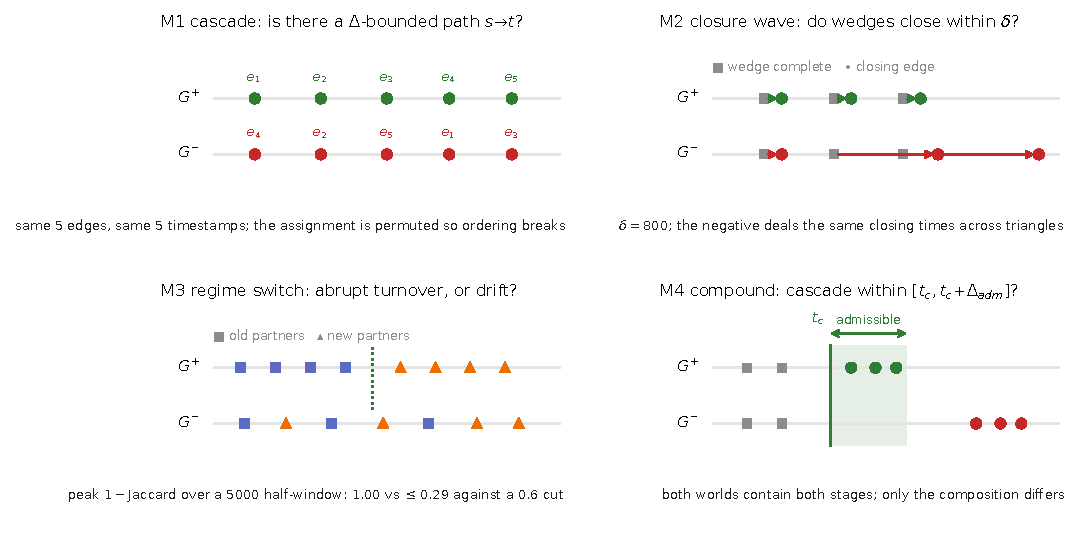
\includegraphics[width=\textwidth]{figures/figure_mechanisms.pdf}
  \caption{\textbf{The four matched counterfactuals.} In every pair the node set, the static edge
  multiset, the event count and the global timestamp multiset are identical; only the assignment of
  timestamps to events differs. M4 additionally guarantees that \emph{both} component predicates
  hold in \emph{both} worlds, so a conjunctive strategy cannot separate the pair.}
  \label{fig:mech}
\end{figure*}

\subsection{Agent interfaces}
\textbf{A0} exposes full-horizon aggregates with no window parameter and serves as the
identifiability control. \textbf{A1} adds a window parameter but no ordering-aware operator; its
burden is information acquisition through interaction. \textbf{A2} exposes raw $(u,v,t)$ events in
a sandboxed Python interpreter with no temporal operators; its burden is algorithm synthesis.
\textbf{A3} exposes semantic temporal operators; its burden is semantic specification and
interpretation. All conditions share one dispatch loop and differ only in the tool surface and a
single prompt paragraph, so the comparison is a statement about the interface rather than about
harness engineering.

\subsection{Models}
\texttt{gpt-5-mini} and Opus~5 as principal subjects, plus an open-weight ladder of
Qwen2.5-Instruct-AWQ at 7B, 14B and 32B, served locally through an OpenAI-compatible endpoint so
that open-weight subjects run a byte-identical agent loop. One family and one quantisation, so
scale is the only variable that moves. A deterministic reconstruction script is included as a
sanity baseline only.

\subsection{Trace instrumentation: citations and reconstruction}
\label{sec:instr}
Two quantities recur throughout the results and are defined here rather than left to narrative
reading. Both are computed deterministically from the stored trace.

\paragraph{Citations and the support set.}
Every tool response is assigned a monotonically numbered step id (\texttt{step\_01},
\texttt{step\_02}, \dots) at the moment it is executed, and the id is shown to the agent alongside
the result. The output contract, identical across all conditions, requires the final answer to be
a JSON object whose \texttt{evidence} field is a list of \texttt{\{trace\_id, role\}} entries with
\texttt{role} $\in$ \{\texttt{support}, \texttt{confounder\_control}\}. We parse that field
directly; nothing is inferred from prose. The support set is
\[
S_i^{\text{support}}=\{\,s : (s,\texttt{support})\in \text{evidence},\; s\in \text{steps}(\tau_i)\,\},
\]
the cited entries that resolve to steps actually present in the trace $\tau_i$. A claim citing an
id that was never executed is recorded as \textbf{fabrication} and cannot contribute support; this
is how the smallest open-weight checkpoint is scored, since it emits well-formed claims citing
steps it never ran. A run with an empty support set is evidence-invalid by construction, because
the existential in $EV_i$ has nothing to range over. Agents may cite several steps, and routinely
do, which is precisely why the existential quantifier matters (\S\ref{sec:threats}).

\paragraph{Reconstruction detection.}
Reconstruction is a rule, not a judgement. A run is marked as using range reconstruction when it
issues at least three successful \texttt{window\_event\_count} calls that are \emph{both}
node-filtered and batched over at least two windows in a single call. That conjunction is the
signature of the batched bisection observed in development: the node filter is what makes a count
informative about a particular pair of endpoints, and multiple windows per call is what makes the
search efficient enough to attempt under a budget. We also record the number of such calls, the
mean windows per call, and the narrowest window width reached, which together give the cost profile
of the strategy. The detector fires on the \emph{attempt}, not on success, which is what allows us
to report that Opus continues to reconstruct at $0.80$--$1.00$ while its accuracy falls to zero.

\subsection{Controls}
Six preregistrations committed before the results they govern; an outcome-independent protocol
gate; per-pair invariant records; content-derived run identifiers; superseded sweeps retained on
disk under explicit names and excluded from analysis; deterministic rescoring and backend replay
from stored traces; and separation of \emph{tool-protocol failure} from \emph{analytical failure}.
The last matters for the open-weight ladder: a model that cannot emit a well-formed tool call has
not been measured on temporal reasoning at all. Across all 270 open-weight episodes we observe
\textbf{zero tool-protocol errors}, so nothing reported below is a formatting artifact.

The corpus is $1{,}402$ scored runs: every episode whose world recompiles to its recorded hash
under the frozen configuration. It \emph{excludes} superseded sweeps; an early sweep invalidated
by a world-naming collision, and the M3 runs predating a preregistered amendment, which remain
on disk under explicit names. Counts quoted elsewhere in this paper are drawn from that same set.
All cells use $5$ paired seeds; the main matrix is at development scale with
\texttt{confounder:none}, plus the two robustness cells of \S\ref{sec:robust}.

%% ===================================================================================
\section{Results}

\begin{figure*}[t]
  \centering
  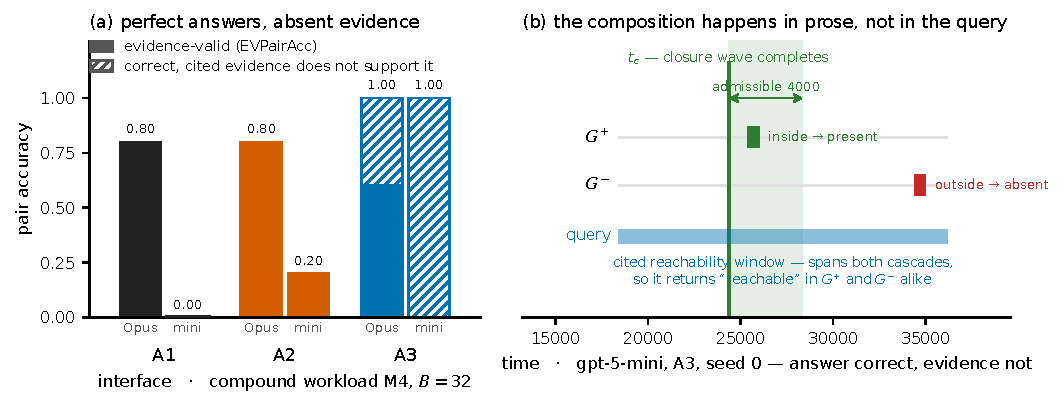
\includegraphics[width=\textwidth]{figures/figure1.pdf}
  \caption{\textbf{The same final answer, different analytical validity.}
  \textbf{(a)} The compound workload M4 at $B{=}32$. Bar height is \pairacc; the solid portion is
  \evpair{}; answers whose cited computation preserved the question's semantics, and the
  hatched remainder is correct answers their own evidence does not support. A1 and A2 show no gap.
  Under A3 both models score $1.00$ while \texttt{gpt-5-mini}'s evidence validity is $0.00$.
  \textbf{(b)} Why, from one real run. The closure wave completes at $t_c{=}24382$ and the
  admissible interval is $[t_c,t_c+\Delta_{\text{adm}}]=[24382,28382]$. The positive world's
  cascade starts at $25382$ (inside); the
  negative world's at $34382$ (outside). The agent's \emph{cited} reachability query spans
  $[18400,36212]$ and therefore returns \emph{reachable} in both worlds: it cannot distinguish the
  case it is offered as establishing.}
  \label{fig:one}
\end{figure*}

\subsection{RQ1: What is the model--interface system capable of?}

\subsubsection{A0 establishes the identifiability floor}
A0 is order-oblivious by exhaustive validation: between 6{,}018 and 13{,}747 distinct A0 queries
per pair return byte-identical responses across $\Gp$ and $\Gm$, on every mechanism. A0 pair
accuracy is $0.00$ for both principal models. Two floors follow. Under observational equivalence a
deterministic policy returns the same decision for both members of a pair and so scores
$\pairacc=0$. For independent randomized prediction with probability $p$ of answering
\emph{present}, expected pair accuracy is $p(1-p)\le0.25$.

\subsubsection{A1 has emergent capability}
Under A1 no operation returns a timestamp or an ordering. Opus~5 nonetheless performs batched
node-filtered range queries that localize events and recover their order, with a reconstruction
rate of $0.80$--$1.00$ at every resolution tested. \emph{The effective capability of an
agent-facing interface can exceed the advertised semantics of its individual operations.}

\subsubsection{M1 exposes an interaction-limited frontier}
Table~\ref{tab:m1} and Figure~\ref{fig:two} give the resolution sweep at $B{=}16$.

\begin{table}[t]
\caption{M1 cascade, $B{=}16$, $k{=}5$, $D{=}0$, 5 seeds. Reconstruction is the share of Opus runs
showing sustained node-filtered localization. A2 and A3 values are $1.00$ for \emph{both} models at every $R$ where they were run;
\textsc{n/r} marks combinations that were not run rather than a missing result. Per-seed outcomes
are shown because $n{=}5$.}
\label{tab:m1}
\small
\begin{tabular}{@{}rcccccc@{}}
\toprule
$R$ & Opus A1 & per-seed & recon. & mini A1 & A2 & A3 \\
\midrule
32  & 1.00 & \texttt{11111} & 0.90 & 0.00 & 1.00 & 1.00 \\
128 & 1.00 & \texttt{11111} & 0.90 & 0.00 & n/r  & 1.00 \\
192 & 0.60 & \texttt{01101} & 0.90 & 0.00 & n/r  & n/r \\
256 & 0.40 & \texttt{01001} & 0.90 & 0.00 & 1.00 & n/r \\
384 & 0.00 & \texttt{00000} & 1.00 & 0.00 & n/r  & n/r \\
512 & 0.00 & \texttt{00000} & 0.80 & 0.00 & 1.00 & 1.00 \\
\bottomrule
\end{tabular}
\end{table}

Two features matter more than the curve itself, and Figure~\ref{fig:two} shows them together.
First, the reconstruction attempt rate does \emph{not} decline: pair accuracy falls while Opus continues to attempt the same strategy in
80--100\% of runs, so the loss coincides with failure to \emph{complete} the strategy inside a
fixed budget rather than with abandoning it. Second, the per-seed success sets are nested and
non-increasing, with strict drops after $R{=}128$:
\[
\{0,1,2,3,4\}\supseteq\{0,1,2,3,4\}\supsetneq\{1,2,4\}\supsetneq\{1,4\}\supsetneq\emptyset .
\]
Individual instances therefore become infeasible progressively rather than at random. We do not
claim nesting alone excludes sampling noise; it does not. The interaction-limited reading rests
on three things jointly: the monotone decline, the persistent reconstruction rate, and M2's
reproduction of the same pattern along a different axis.
The pooled contrast $R\le256$ versus $R>256$ is $+0.75$ (95\% CI $[+0.55,+0.95]$, 10k paired
bootstrap), the only interval we report. \texttt{gpt-5-mini} never separates a pair at any $R$ and
attempts reconstruction in $0.13$ of runs.

\subsubsection{M2 reproduces the frontier through budget}
Varying the budget instead of the search range reproduces the pattern on a different mechanism:
Opus A1 rises from $0.00$ at $B{=}8$ (reconstruction $0.60$) to $0.60$ at $B{=}32$ (reconstruction
$1.00$), while \texttt{gpt-5-mini} stays at $0.00$. The frontier is a property of the
model--interface--resource system, not of temporal reasoning in the abstract.

\subsubsection{A2 localizes the bottleneck as acquisition}
Given raw events and an interpreter, both models reach $1.00$ at every tested resolution
($R\in\{32,256,512\}$), and on M2 Opus reaches $1.00$ at both budgets with \texttt{gpt-5-mini} at
$0.80$. A2 has strictly more information than A1 and no temporal semantics at all. The A1 frontier
is therefore localized, \emph{for M1}, to the information-acquisition constraints of that interface
rather than to an inability of the tested models to compute the temporal predicate once raw events
are available. This programmable control rules out the simpler explanation that A1 fails because
the predicate itself is beyond the models' reach.

\subsubsection{Model scale does not explain A1 reconstruction}
A naive account predicts $7\text{B} < 14\text{B} < 32\text{B} < \text{Opus}$ under A1. That is not
what happens (Table~\ref{tab:ladder}): all three open checkpoints sit at the floor at every
resolution, while Opus reconstructs. Under A3 the ladder is non-decreasing with checkpoint size in
the tested cells ($0.00\to0.80\to1.00$ on M1 at $R{=}32$, with 7B and 14B tied at $0.80$ on M2),
a far clearer size-related progression than A1 shows.

\begin{table}[t]
\caption{Open-weight ladder, Qwen2.5-Instruct-AWQ, 270 episodes, zero tool-protocol errors. Fab.\
is the fabrication rate on the A3 M1 cells: the share of runs emitting a well-formed claim citing
steps that were never executed.}
\label{tab:ladder}
\small
\begin{tabular}{@{}lccccc@{}}
\toprule
 & A1 (all $R$) & A3 $R{=}32$ & A3 $R{=}512$ & A3 M2 & Fab. \\
\midrule
7B  & 0.00 & 0.00 & 0.00 & 0.80 & 1.00 \\
14B & 0.00\,$^{\dagger}$ & 0.80 & 1.00 & 0.80 & 0.20--0.30 \\
32B & 0.00 & 1.00 & 1.00 & 1.00 & 0.00 \\
\bottomrule
\multicolumn{6}{@{}l@{}}{\footnotesize $^{\dagger}$ one cell at $R{=}256$ reaches 0.20.}
\end{tabular}
\end{table}

We therefore avoid the claim that larger models push the frontier outward. The supported statement
is that \emph{different models occupy qualitatively different strategy regimes under the same
low-level interface, and size alone does not predict whether adaptive reconstruction emerges}. The
contrast with A3 is the informative part: semantic operators convert the task from strategy
invention into interpretation, and interpretation does scale here where strategy invention did not.
The 7B failure is not an inability to call tools; protocol errors are zero and it uses tools
correctly on M2, but fabrication: on M1+A3 it makes \emph{zero} tool calls and emits claims
citing steps that never existed, at a rate of $1.00$.

\subsection{RQ2: When the system succeeds, is the analysis valid?}

\subsubsection{The gap appears only under semantic operators}
Under our deterministic task-constraint checker we observe \emph{no} \pairacc--\evpair{} gap for
A1 or A2 in any tested cell, for either model. A3 exhibits substantial gaps on M1, M2 and
especially M4 for at least one principal model, while M3 exposes a \emph{different} semantic-stage
failure rather than a gap: \texttt{gpt-5-mini} obtains task-consistent operator evidence and
misinterprets it, so its M3 accuracy and evidence validity are equal and both low
(Table~\ref{tab:gap}). This is an observation about the tested cells and this
checker; it is not proof that arbitrary A1 or A2 reasoning is semantically valid. Their gap is
also zero partly because A1 rarely succeeds, and because a program that ignores a stated bound
usually prints something visibly wrong that the agent then repairs.

\begin{table}[t]
\caption{The A3 evidence gap, reported \emph{per mechanism} at the headline cells rather than as a
pooled average. Pooling would weight mechanisms by how many cells each happens to have; the
ambiguity sweep alone contributes 20 cells for \texttt{gpt-5-mini} and none for Opus, so the
two models would not be comparable. Each entry is 5 paired seeds per model except M1, which pools
$R\in\{32,128,512\}$ (15 pairs). A1 and A2 show no gap in any tested cell and are omitted.}
\label{tab:gap}
\small
\begin{tabular}{@{}lcccc@{}}
\toprule
& \multicolumn{2}{c}{Opus 5} & \multicolumn{2}{c}{gpt-5-mini} \\
\cmidrule(lr){2-3}\cmidrule(lr){4-5}
mechanism & \pairacc & \evpair & \pairacc & \evpair \\
\midrule
M1 cascade       & 1.00 & 0.67 & 1.00 & 0.53 \\
M2 closure wave  & 1.00 & 0.20 & 1.00 & 0.80 \\
M3 regime switch & 1.00 & 0.60 & 0.20 & 0.20 \\
M4 compound      & 1.00 & \textbf{0.60} & 1.00 & \textbf{0.00} \\
\bottomrule
\end{tabular}
\end{table}

\subsubsection{M3 reveals interpretation failure}
\label{sec:m3}
On M3, \texttt{gpt-5-mini} under A3 scores $0.20$ against Opus's $1.00$, and the traces show the
failure is not acquisition. It invokes the intended operator with the task's own parameters and
receives a decisive number: the negative worlds return a peak change of $0.210$--$0.286$ against
positives at $1.000$. It then answers \emph{present} on four of five negatives, narrating over the
raw contact lists the operator also returns. Opus mis-parameterises \emph{more} often ($0.18$ of
temporal calls versus $0.05$) and is nonetheless correct, because it cross-checks rather than
reading a single number. Information availability plus a correct semantic query does not imply
correct interpretation.

\subsubsection{M4: perfect accuracy with no valid support}
Figure~\ref{fig:one} and Table~\ref{tab:m4} give the compound workload. Both models reach $1.00$
under A3; \evpair{} is $0.60$ for Opus and $0.00$ for \texttt{gpt-5-mini}. A1 and A2 again show no
gap.

\begin{table}[t]
\caption{M4 compound, $B{=}32$, 5 seeds. Calls is the mean number of tool calls per episode.}
\label{tab:m4}
\small
\begin{tabular}{@{}llccc@{}}
\toprule
interface & model & \pairacc & \evpair & calls \\
\midrule
A1 & Opus 5     & 0.80 & 0.80 & 32.0 \\
A1 & gpt-5-mini & 0.00 & 0.00 & 26.9 \\
A2 & Opus 5     & 0.80 & 0.80 & 12.1 \\
A2 & gpt-5-mini & 0.20 & 0.20 & 3.6 \\
A3 & Opus 5     & \textbf{1.00} & 0.60 & 7.8 \\
A3 & gpt-5-mini & \textbf{1.00} & \textbf{0.00} & 2.4 \\
\bottomrule
\end{tabular}
\end{table}

The mechanism is visible in Figure~\ref{fig:one}(b). \texttt{gpt-5-mini} issues a reachability
query over an interval wider than the admissible lag. That query returns \emph{reachable} in both
matched worlds by construction, so it cannot separate the pair, yet the model reaches the
correct conclusion by reasoning over the returned arrival times in prose. Opus cites such an unbound query in $30\%$ of runs; in the remainder it issues and cites a query
over exactly $[t_c,t_c+\Delta_{\text{adm}}]$. Both models can reach the correct compound conclusion
in their generated reasoning, but the temporal composition is reflected in the \emph{cited}
computation only intermittently for Opus and never for \texttt{gpt-5-mini} in the tested pairs.
Note that per-run and per-pair rates differ by construction: both members of a pair must be
evidence-valid, so a $30\%$ per-run invalid rate yields a $0.40$ pair-level gap.

\subsubsection{Cost: efficiency does not imply validity}
Table~\ref{tab:cost} separates the three cost families. Backend figures come from serial replay of
recorded tool calls against recompiled worlds, with no LLM and no API cost, because the sweeps ran
at concurrency 8--12 and their wall-clock is contaminated by queueing.

\begin{table}[t]
\caption{Cost decomposition, averaged over \emph{all} valid runs of each (model, interface) pair
across M1--M4 and every budget. These are global observed averages over unequal mixes of mechanisms
and budgets, not matched comparisons; the equal-accuracy comparison is in the text. Events/LLM is
the number of events the data system examined per LLM round. Latency is measured separately at
concurrency 1.}
\label{tab:cost}
\small
\begin{tabular}{@{}llccrr@{}}
\toprule
model & int. & LLM calls & \$/run & events/LLM & backend ms \\
\midrule
Opus 5 & A1 & 7.6 & 0.414 & 107{,}326 & 21 \\
Opus 5 & A2 & 8.3 & 0.399 & 17{,}571 & 1349 \\
Opus 5 & A3 & \textbf{6.2} & \textbf{0.298} & 25{,}897 & 32 \\
\addlinespace
gpt-5-mini & A1 & 9.3 & 0.021 & 34{,}697 & 12 \\
gpt-5-mini & A2 & \textbf{3.7} & 0.011 & 11{,}761 & 1209 \\
gpt-5-mini & A3 & 5.1 & \textbf{0.007} & \textbf{9{,}445} & 10 \\
\bottomrule
\end{tabular}
\end{table}

In the controlled equal-accuracy comparison for Opus, A3 uses fewer interactions, lower API cost
and lower end-to-end latency than A1 and A2, with concurrency-1 latency of $64.3$\,s, $24.9$\,s and
$20.8$\,s per episode respectively. Backend-work comparisons depend on the metric: A2 scans the
fewest events per LLM round and A3 the least backend time, while A1 scans by far the most, which is
reconstruction made visible as backend work.

One negative result deserves emphasis because it is easy to misreport: A2's $\approx$1.3\,s backend
time is \emph{our harness}, not the interface. A \texttt{run\_python} call with an empty program
costs $81.0$\,ms and a real reachability program $84.7$\,ms, so the computation is $\approx$4\,ms
and the remainder is process-per-call spawn and serialisation. The engine-independent measure is
events scanned, by which A2 is cheaper than A1. \emph{The cheapest and most accurate trajectory can
still be semantically invalid.}

\begin{figure*}[t]
  \centering
  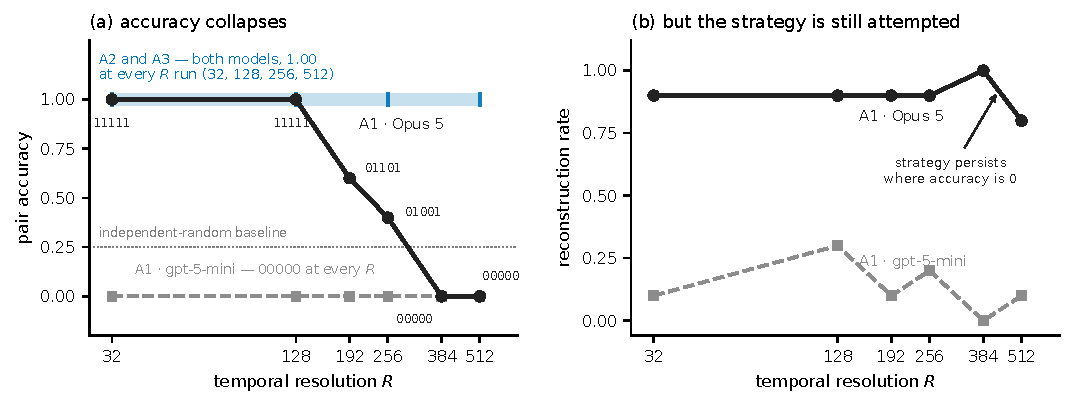
\includegraphics[width=\textwidth]{figures/figure2.pdf}
  \caption{\textbf{The frontier is interaction-limited, not comprehension-limited.} M1 cascade,
  $B{=}16$, 5 seeds. \textbf{(a)} Pair accuracy against the task-relative search range. Opus~5
  under A1 falls from $1.00$ to $0.00$ across a $16\times$ growth in $R$ while
  \texttt{gpt-5-mini} never separates a pair; per-seed outcomes are printed because $n{=}5$. Both
  abstractions remove the frontier at every $R$ they were run at. \textbf{(b)} The reconstruction
  rate over the same cells. The detector fires on the \emph{attempt}, never on success, and Opus
  keeps attempting the same strategy at $0.80$--$1.00$ precisely where its accuracy is zero. The
  two panels coming apart is the evidence for a resource boundary: what degrades is completion
  inside a fixed budget, not the discovery of the strategy. \texttt{gpt-5-mini} is categorically
  different, attempting reconstruction in $0.00$--$0.30$ of runs throughout.}
  \label{fig:two}
\end{figure*}

\subsubsection{Robustness: the A1 frontier moves with event volume}
\label{sec:robust}
Two preregistered robustness cells at $R{=}128$, where Opus+A1 scores $1.00$ at baseline, test
whether the frontier is an artifact of our nuisance conditions or our world size
(Table~\ref{tab:robust}).

\begin{table}[t]
\caption{Robustness cells, M1 at $R{=}128$, $B{=}16$, 5 seeds. \emph{Confounder} overlays a broad
activity spike ($\approx${+}20\% events) applied \emph{identically} to both worlds, so it carries
no pair-discriminating information. \emph{Scale} raises the graph from 2{,}000 to 8{,}000 nodes
($\approx4\times$ events).}
\label{tab:robust}
\small
\begin{tabular}{@{}llccc@{}}
\toprule
condition & model & A1 & A3 & A1 calls \\
\midrule
baseline          & Opus 5     & 1.00 & 1.00 & 12.6 \\
+ confounder      & Opus 5     & \textbf{0.60} & 1.00 & 16.0 \\
+ scale (8K)      & Opus 5     & \textbf{0.80} & 1.00 & 16.0 \\
\addlinespace
baseline          & gpt-5-mini & 0.00 & 1.00 &; \\
+ confounder      & gpt-5-mini & 0.00 & 1.00 & 12.4 \\
+ scale (8K)      & gpt-5-mini & 0.00 & 1.00 & 14.4 \\
\bottomrule
\end{tabular}
\end{table}

Both cells degrade Opus under A1 and neither touches A3. We had predicted the confounder would be
inert, since its events are identical across the pair and therefore cannot be discriminative; that
prediction was wrong, and the reason is instructive. In both degraded cells Opus consumes exactly
$16.0$ calls (the budget ceiling) while its reconstruction rate stays at $0.90$. The
trace statistics are consistent with increased search cost rather than a change of strategy: the
additional activity increases the event mass each range probe must disambiguate. We did not verify
by trace inspection that the agent never follows the burst as a shortcut, so we do not claim the
confounder \emph{cannot} mislead; only that these traces do not look like it. The same reading
applies to the scale cell.

The A1 frontier therefore moves with the volume of events that must be searched, whether that
volume comes from temporal span ($R$), graph size, or nuisance activity, while A3 remains at $1.00$
in the tested $R$, confounder and scale cells. This bounds the $R$ curve ($R$ is not the only axis that moves the frontier) and
supports the interaction-limited reading of it. \emph{Scale here is a robustness check, not a
scalability study}: $2\text{K}\to8\text{K}$ shows the behavior is not an artifact of a small
graph, nothing more.

\subsection{Summary}
Figure~\ref{fig:framework} maps each result to the stage it exposes: A0 to identifiability, A1
under M1 and M2 to strategy formation and completion, A2 to the localization of that frontier as
acquisition, M3 to evidence interpretation, and M4 to intent-to-execution validity. The
mechanism-level accuracy and validity numbers are in Tables~\ref{tab:m1}--\ref{tab:robust}.

%% ===================================================================================
\section{Discussion}

Read against the staged profile, the four interfaces fail in four different places, and that is the
synthesis this paper offers. A0 fails at stage one: no permitted query separates the pair, so no
amount of model capability helps and pair accuracy is $0.00$ by information rather than by
inability. A1 moves the difficulty to stages two and three: the information is present but only indirectly, so
the agent must invent a reconstruction strategy and then finish it inside a budget, and a frontier
model does the first reliably and the second only while the search range stays small. A2 dissolves
both stages by handing over the events, showing that what A1 measured was acquisition rather than
temporal reasoning. A3 dissolves them differently, by computing the relation directly, and thereby
exposes the two stages abstraction cannot remove: M3 shows a model receiving a decisive number and
misreading it, M4 a model reaching correct conclusions on computations that cannot establish them.
Moving intelligence into the interface does not remove work. It moves \emph{where the work and the
failure live}, and the later stages are the ones that answer accuracy cannot see.

None of this argues against semantic operators. A3 was the most accurate, cheapest, fastest and
most interaction-efficient interface we tested for the frontier model, and on three of four
mechanisms it lifted a substantially cheaper model to the same accuracy. The evidence-validity gap
is an argument for semantic interfaces with stronger intent-to-execution validation, not for
abandoning abstraction: operators that make the relationship between a stated constraint and the
executed computation checkable, so a mis-aimed call is visible at the interface rather than only in
a later trace audit. A2 shows the choice is not binary either, and the interesting design question
is which of programmable access, semantic operators and plan validation owns each stage.

The methodology transfers beyond temporal graphs. It applies wherever an agent interacts with a
structured analytical API and the ground truth can be manipulated while nuisance statistics are
held fixed. A database study could vary join or aggregation interfaces; a provenance system could
test whether aggregate access reconstructs evidence that was meant to be hidden; a scientific
workflow could replace temporal constraints with experimental conditions. In each case the two
questions are the same as ours: what distinctions can this model--interface system recover, and
does the computation it cites establish the proposition the user asked about?
%% ===================================================================================
\section{Threats to Validity}
\label{sec:threats}

\paragraph{External validity.}
Every mechanism is planted in a synthetic background, so while M4 is compositionally realistic it
is not a validation against real topology, and we make no claim that these worlds resemble any
particular deployed graph. The main matrix runs at development scale with
\texttt{confounder:none}; the two robustness cells of \S\ref{sec:robust} widen that only slightly,
adding a global-burst overlay and an $8{,}000$-node world at a single resolution. Both degrade A1
and leave A3 untouched, which is reassuring, but one bait from one of three implemented confounder
families at one value of $R$ cannot exclude the possibility that a different nuisance or a
different cell behaves differently. The $2\text{K}\to8\text{K}$ comparison is a robustness check
that our conclusions are not an artifact of a small graph, not a scalability study, and should not
be read as one. Finally, each mechanism was exercised with a single paraphrase of its question,
even though two were written; wording robustness is therefore untested, and an agent's sensitivity
to phrasing could plausibly interact with the interface in ways we would not have seen.

\paragraph{Measurement validity.}
$\mathrm{SemValid}$ is a deterministic task-constraint-consistency proxy and each of its
interface-specific checks is a \emph{necessary} condition on the cited support rather than a
sufficient one. For semantic operators it compares call arguments against the task's stated
constraints; for the programmable interface it asks only whether a cited program references the
stated bound, not whether the program is correct; for the compound workload it verifies that a
cited query narrowed to an interval no wider than the admissible lag, without confirming that the
interval sat at the right $t_c$. A failure is therefore strong evidence and a pass is weaker, which
makes the metric permissive and makes \texttt{gpt-5-mini}'s $\evpair=0.00$ on M4 the more striking:
none of its cited support satisfies even this weak necessary condition. The rule itself was
corrected once during analysis. Preliminary versions treated \emph{every} cited call as decisive
and so scored ordinary reconnaissance as invalidating, reporting a $0.76$ gap for Opus under A2 and
$1.00$ under A3 on M4; both dissolved under inspection because the decisive computation was present
in the citation list all along. All reported numbers use the corrected existential rule and were
recomputed from stored traces without re-running an episode. One limitation is intrinsic rather
than fixable: we score the computation an agent \emph{cites}, so a correct chain of private
reasoning that is never reflected in a cited call is invisible to us, which is precisely the
situation Figure~\ref{fig:one}(b) documents.

\paragraph{Statistical and model scope.}
Most cells use five paired seeds. We therefore show raw per-seed outcomes throughout rather than
summary statistics alone, report a single preregistered interval, and avoid quoting the transition
midpoint as though it were precisely estimated. That interval, the pooled $R\le256$ versus $R>256$
contrast, is computed with a cluster bootstrap over seeds rather than over $(R,\text{seed})$ cells,
because the same five matched pairs recur at every resolution and treating their outcomes as
independent would understate the uncertainty. Two proprietary models are two points, and the
open-weight ladder mitigates this without removing it: three checkpoints from one family at one
quantization tell us about that family, and the strategy-regime discontinuity we observe under A1
is exactly the kind of result that could differ elsewhere. We accordingly phrase every
model-dependent finding as a property of the tested model--interface--resource system rather than
of model capability in general.
%% ===================================================================================
\section{Conclusion}
Agentic analytical systems are not described adequately by the capabilities of their language
models or by the functions listed in their APIs. Their behavior emerges from information access,
model strategy, execution resources, semantic abstraction and evidence use. Using matched temporal
counterfactuals we show that low-level aggregate interfaces can acquire effective temporal
capability through adaptive composition, that this capability has model- and resource-dependent
frontiers, that programmable raw access removes the acquisition bottleneck, and that semantic
operators improve accuracy, cost and latency. Yet semantic abstraction imposes its own requirement:
the executed analysis must faithfully represent the intended constrained question, and the model
must interpret the returned evidence correctly. On a compound workload one model attains perfect
pair accuracy and zero evidence-valid pair accuracy; right conclusions, unsupported by the
computations it cites. Capability and validity must be evaluated separately, and agent-facing
analytical interfaces should be designed to make the relationship between intent, computation and
cited evidence explicit and verifiable.

%% ===================================================================================
\section{Ethical Considerations}
Temporal graph analysis supports fraud, security, communication, epidemiological and coordination
studies. A detected pattern is not evidence of causation or intent, and we use controlled synthetic
worlds specifically to avoid individual-level claims. Our reliability finding generalizes beyond
temporal graphs: a correct agent conclusion may rest on a computation that does not establish the
requested proposition. High-consequence deployments should require explicit analytical provenance,
semantic validation, and human review.

\bibliographystyle{ACM-Reference-Format}
\bibliography{refs}

\end{document}
